\section{Discussion}\label{Discussion}
\subsection{How auscultation works?}
Heart sounds carry essential physiological information related to the heart's ability to pump blood. This paper analyzes the time-frequency characteristics of heart sounds by utilising short-term Fourier transforms. The primary auscultation area of interest is the mitral valve, situated at the point of the strongest apical beat.

In Fig.\ref{FIG:Time&Frequency.a}, the stable S1 amplitude is primarily concentrated within the 100 Hz frequency range. The aortic valve, located in the second intercostal space of the right sternal border, is further from the heart compared to the mitral valve. It is significantly influenced by lung sounds and exhibits lower amplitude. On the other hand, the pulmonic valve, situated in the second intercostal space of the left sternal border, demonstrates signal characteristics falling between those of the mitral and aortic valves.

This study involved the collection of mitral valve heart sounds from the same patient before and after receiving initial medical intervention, as depicted in Fig. \ref{FIG:Time&Frequency.d} and Fig.\ref{FIG:Time&Frequency.e}. In comparison to healthy subjects, the amplitudes of S1 are found to be unstable, accompanied by noisy lung sounds. However, following the initial treatment, which took place two days later, there was a noticeable improvement. The heart sound cycle becomes clearer, and the energy amplitude of S1 is more pronounced.
\begin{figure*}[htbp]
\centering
    % 插入第一张子图
    \begin{subfigure}{.3\linewidth}
        \centering
        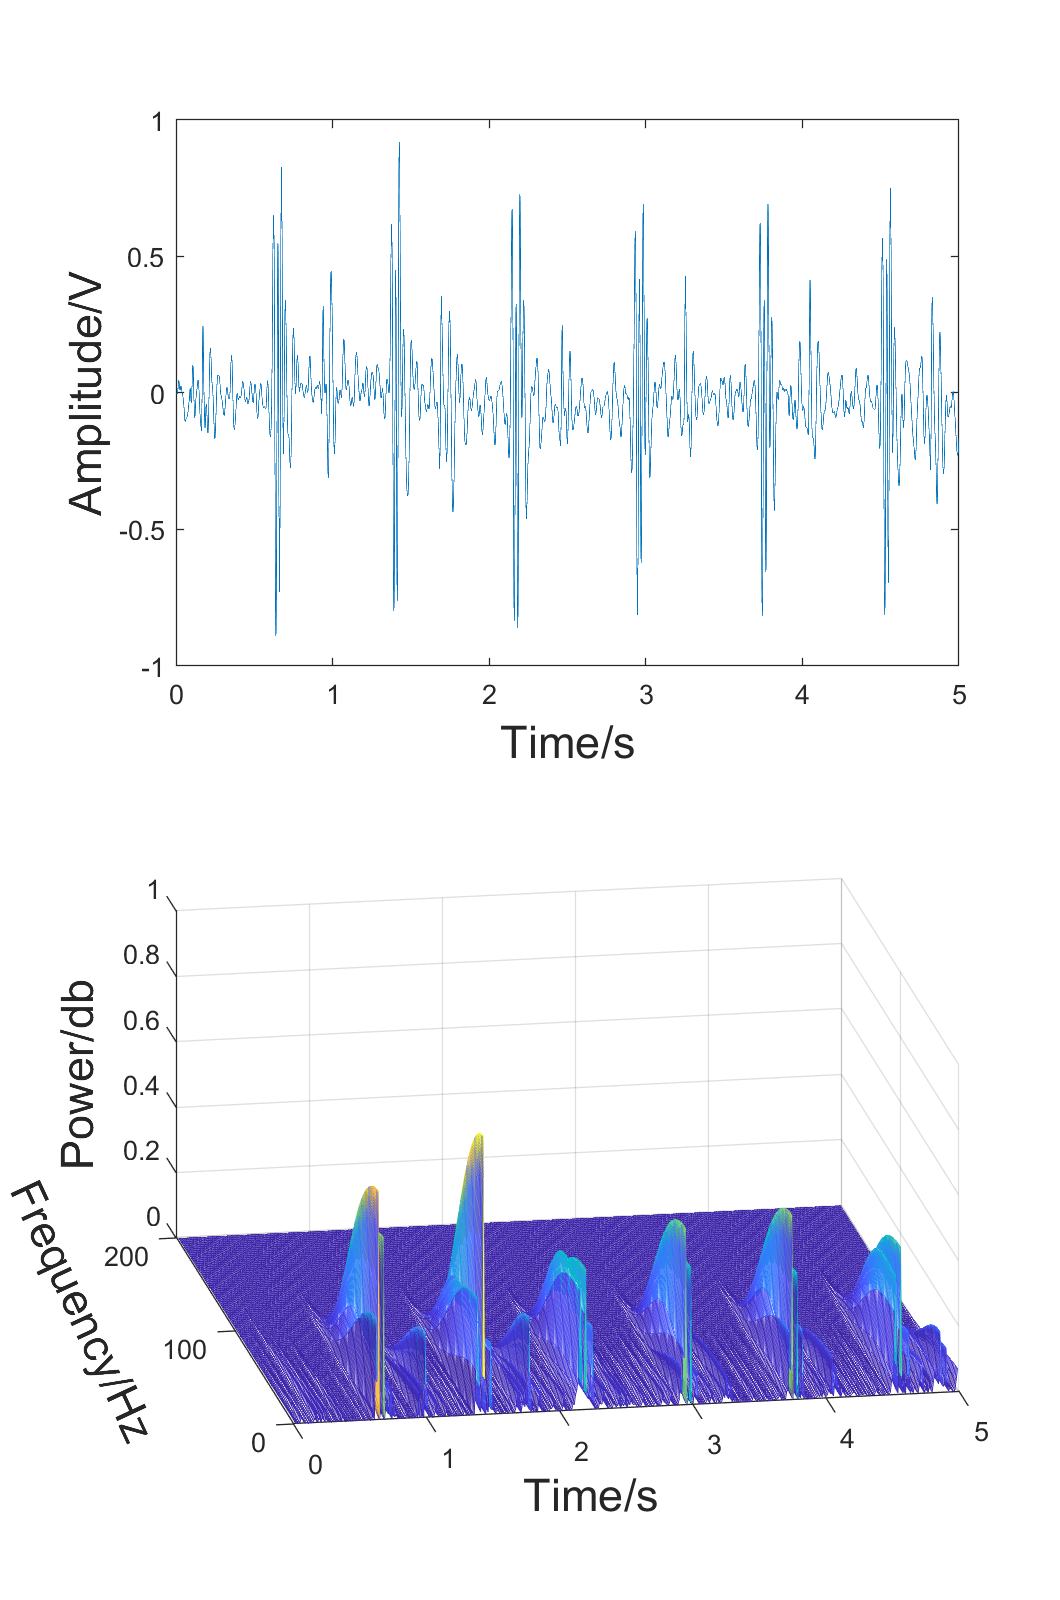
\includegraphics[width=1\linewidth]{figs/disscussion/a.png}
        \caption{Mitral valve}
        \label{FIG:Time&Frequency.a}
    \end{subfigure}\hfill
    % 插入第二张子图
    \begin{subfigure}{.3\linewidth}
        \centering
        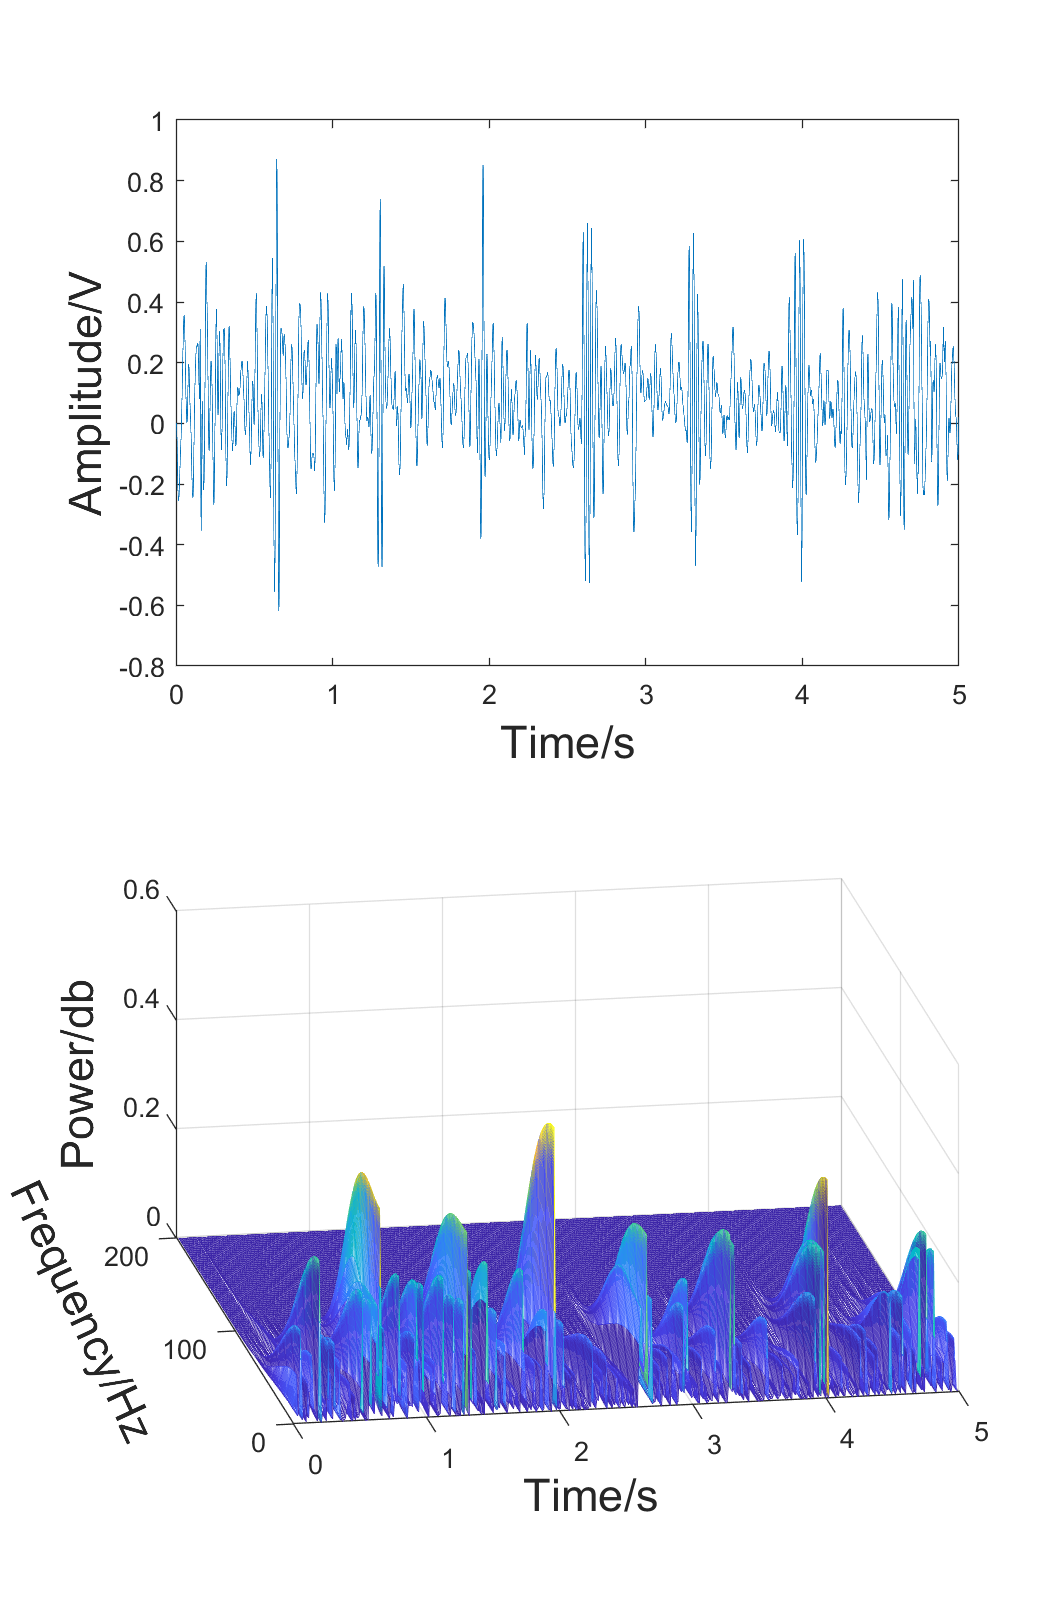
\includegraphics[width=1\linewidth]{figs/disscussion/b.png}
        \caption{Aortic valve}
        \label{FIG:Time&Frequency.b}
    \end{subfigure}\hfill
    \begin{subfigure}{.3\linewidth}
        \centering
        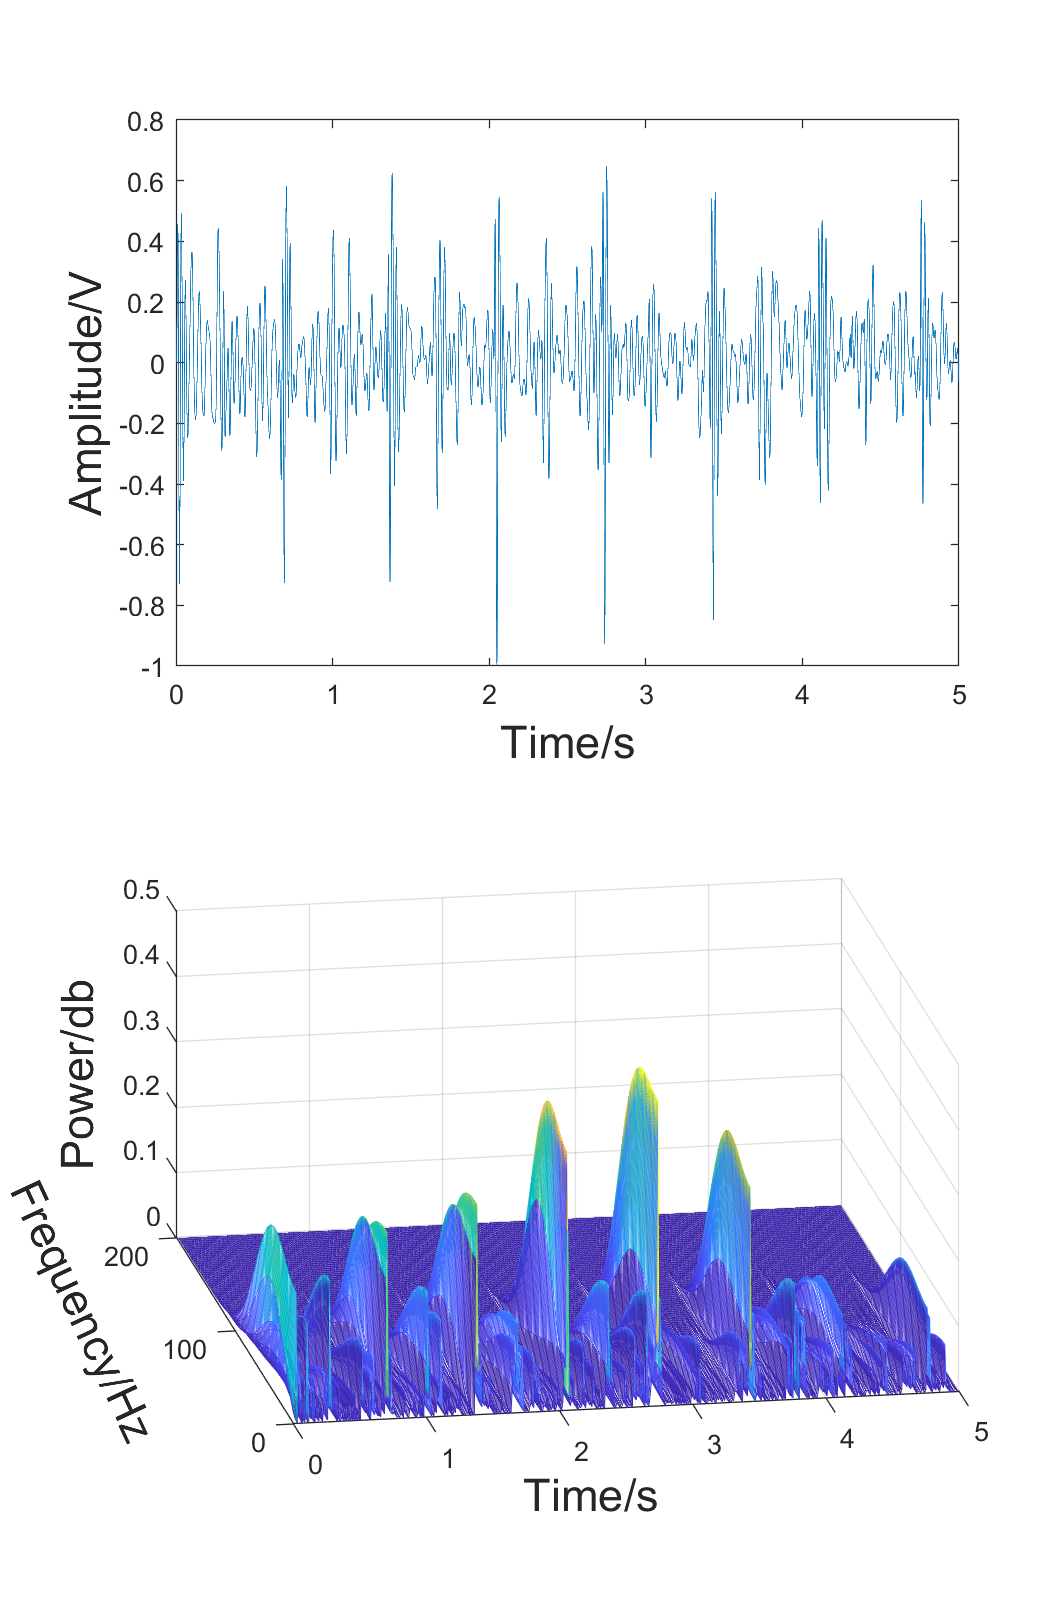
\includegraphics[width=1\linewidth]{figs/disscussion/c.png}
        \caption{Pulmonic valve}
        \label{FIG:Time&Frequency.c}
    \end{subfigure}\\
    \begin{subfigure}{.45\linewidth}
        \centering
        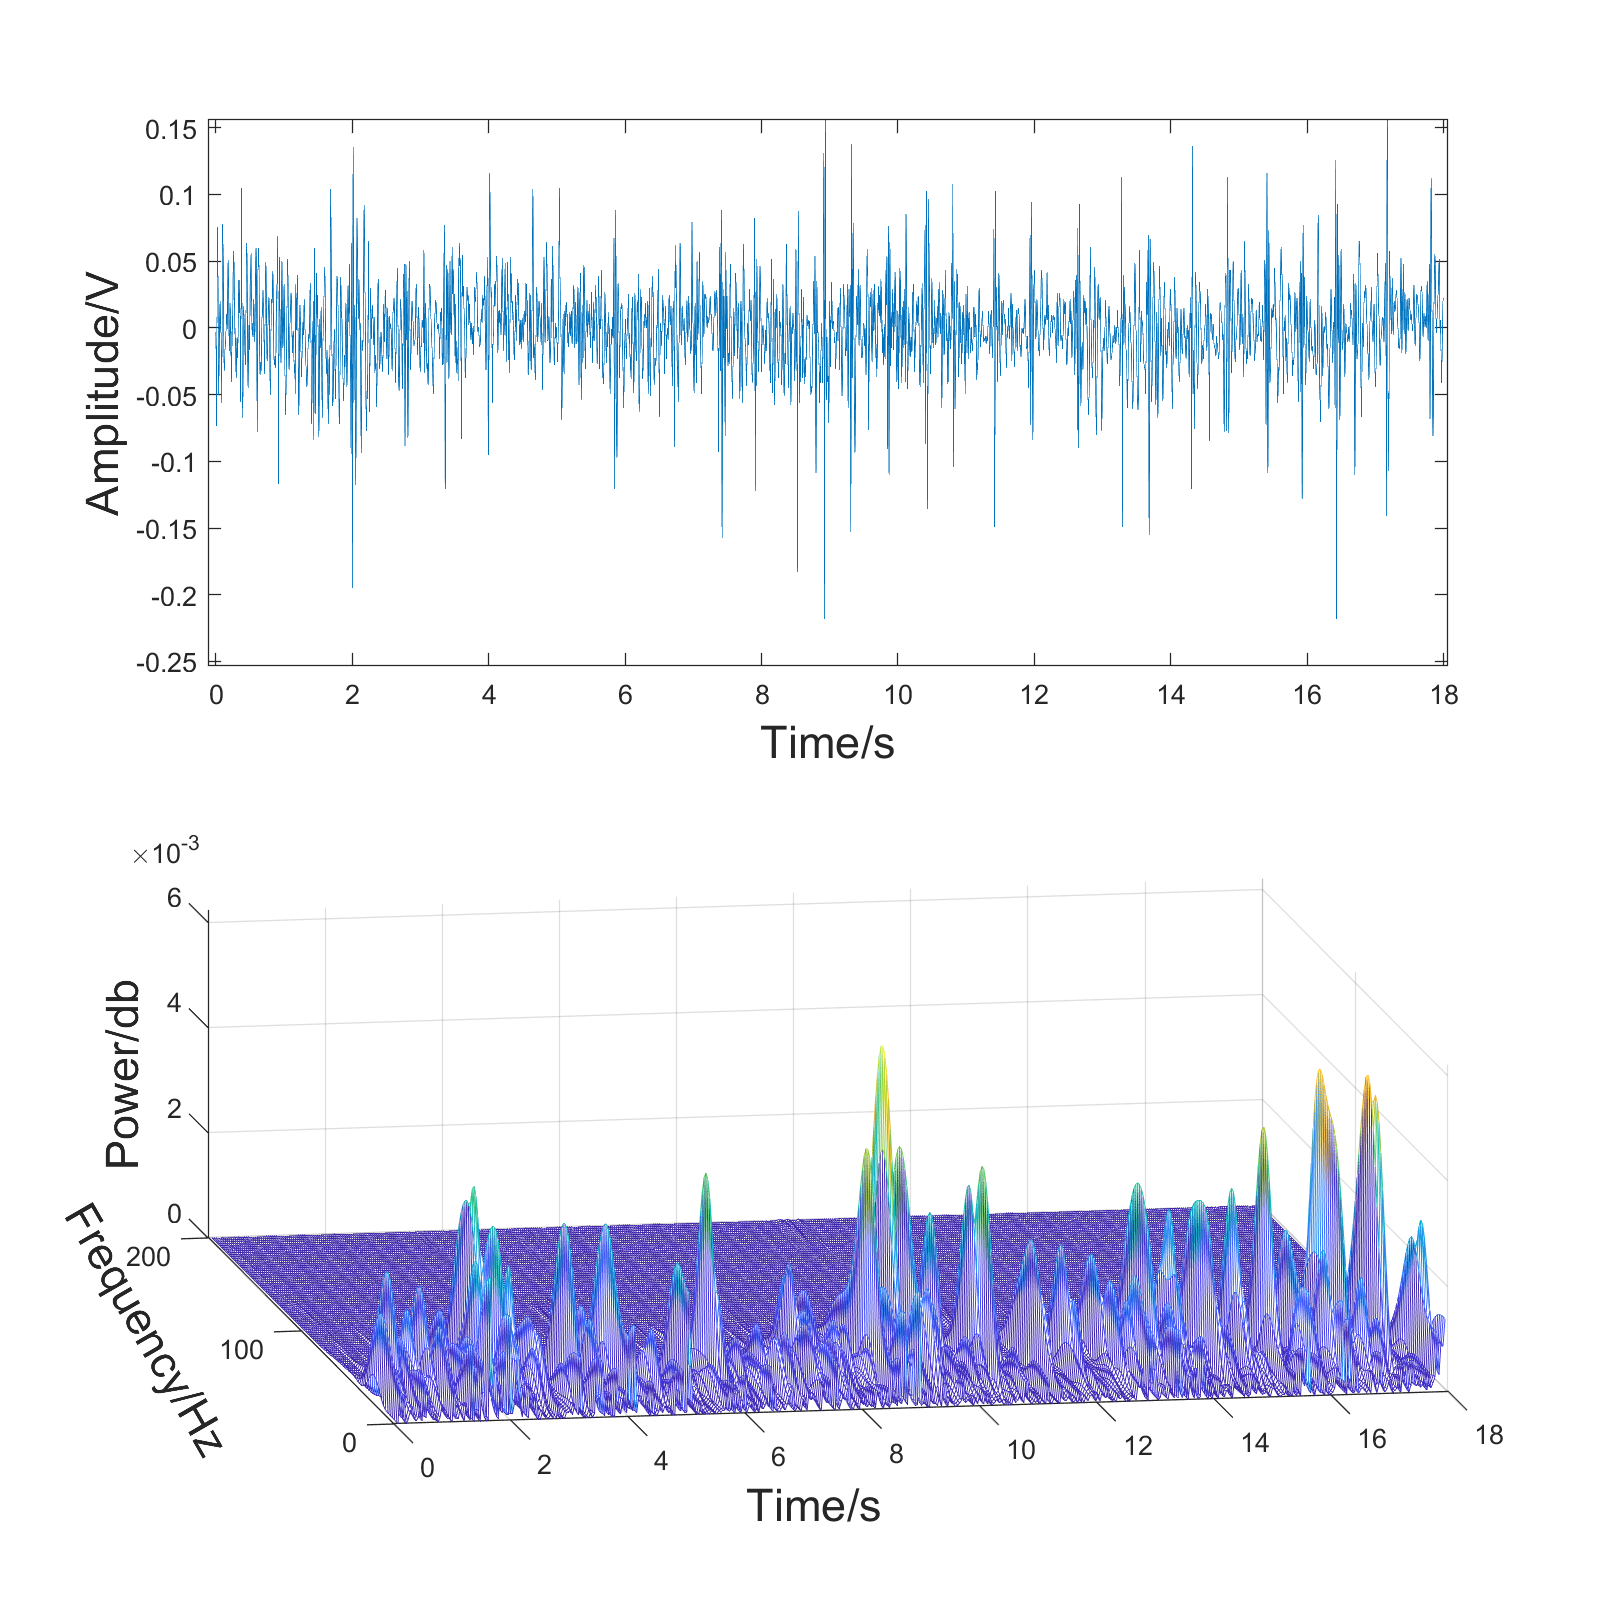
\includegraphics[width=1\linewidth]{figs/disscussion/d.png}
        \caption{Before first-aid}
        \label{FIG:Time&Frequency.d}
    \end{subfigure}\hfill
    % 插入第二张子图
    \begin{subfigure}{.45\linewidth}
        \centering
        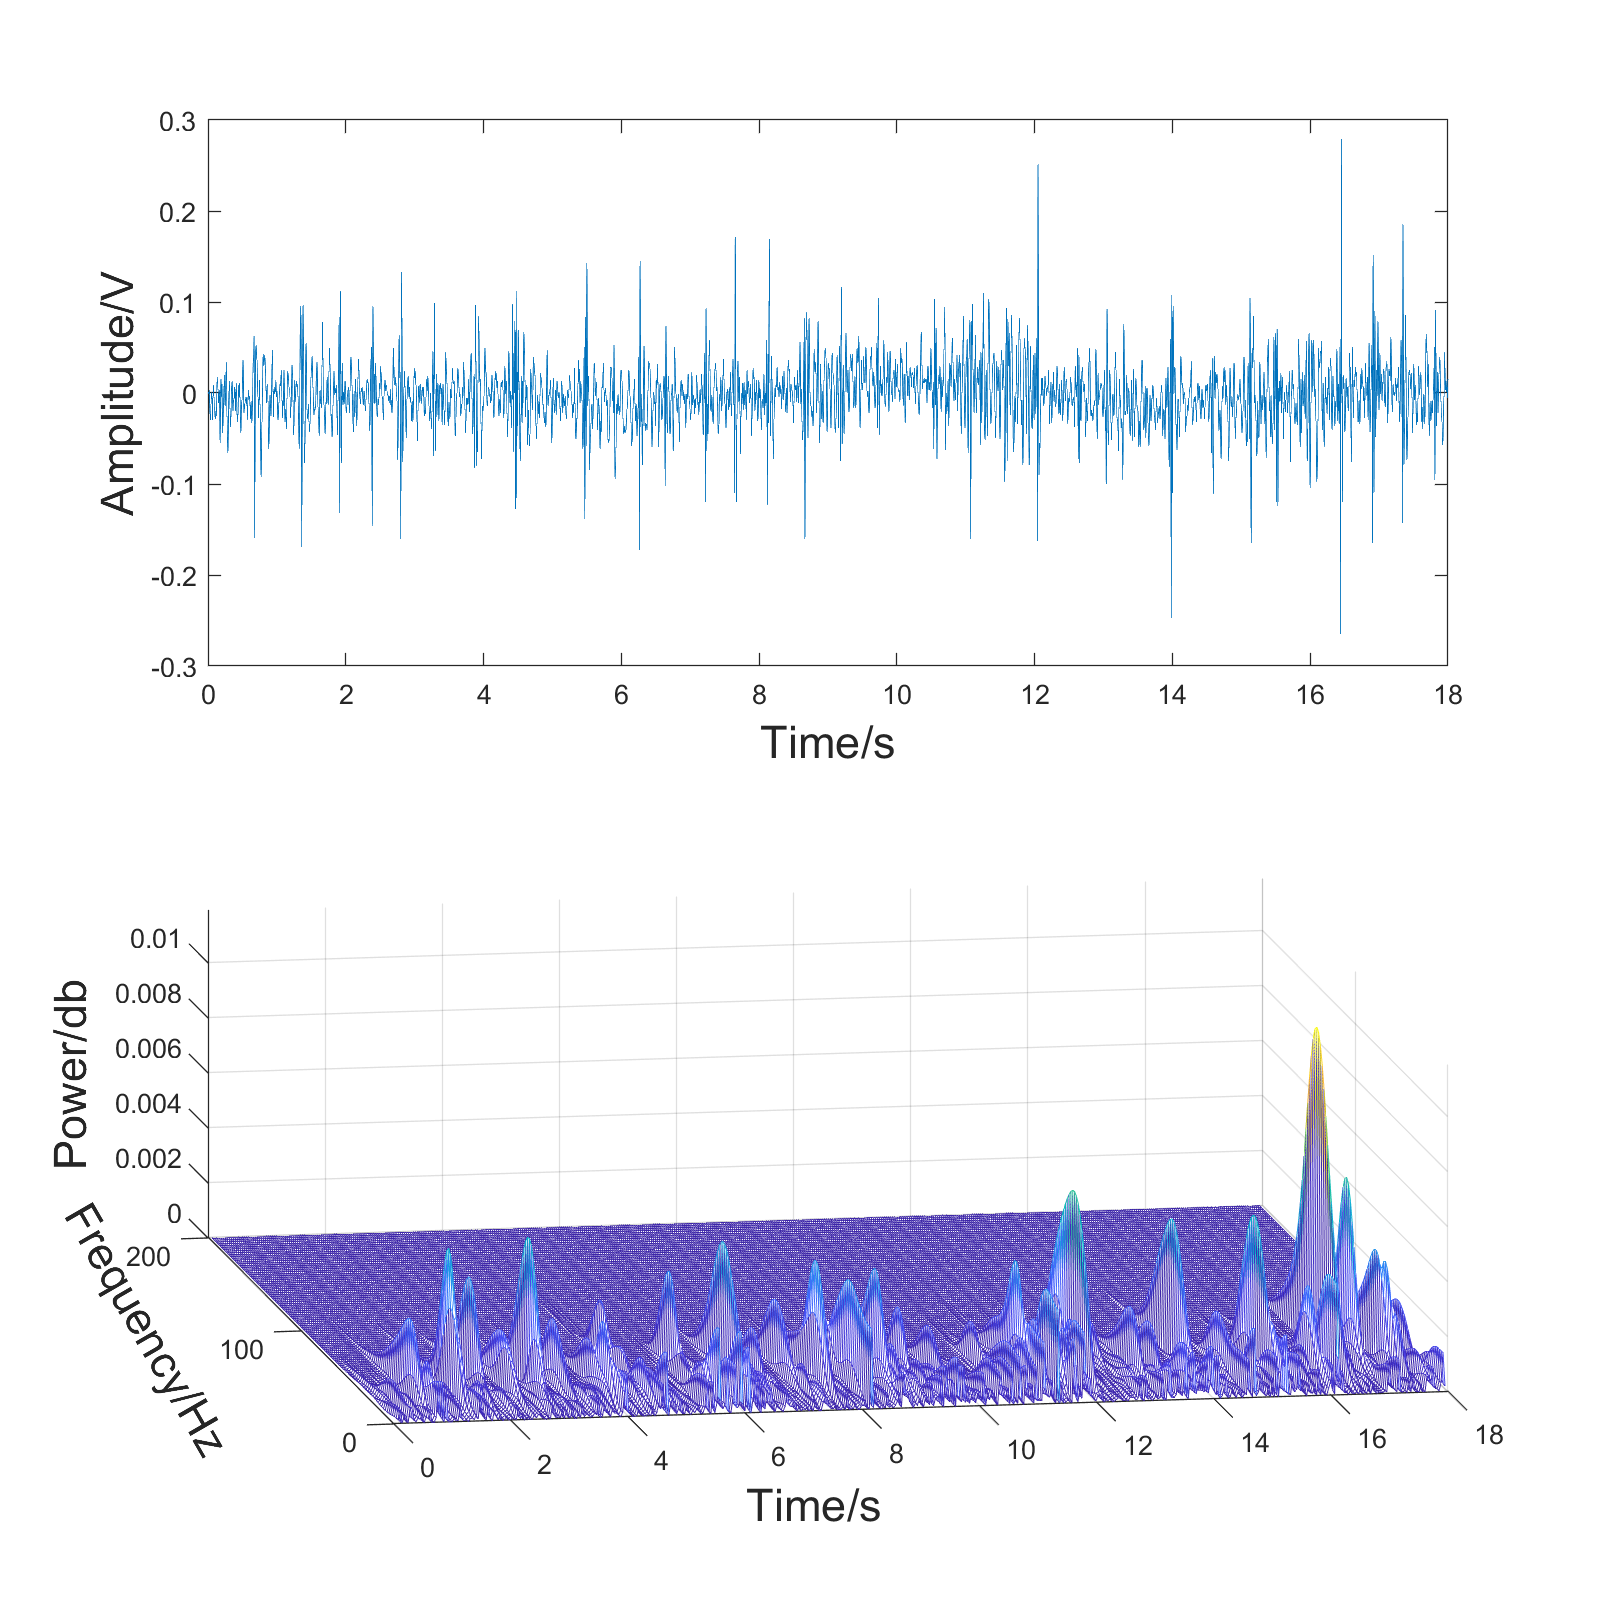
\includegraphics[width=1\linewidth]{figs/disscussion/e.png}
        \caption{After first-aid}
        \label{FIG:Time&Frequency.e}
    \end{subfigure}
\caption{\textbf{Heart sounds in five different situations.} (\textbf{a}) Heart sounds from the mitral valve. (\textbf{b}) Heart sounds from the aortic valve. (\textbf{c}) Heart sounds from the pulmonic valve. (\textbf{d}) Heart sounds before first-aid. (\textbf{e}) Heart sounds after first-aid.}
\label{FIG:Time&Frequency}
\end{figure*}
\subsection{How long should auscultate for?}
The optimal input length for heart sounds in AI models is a subject of debate. Cardiac auscultation offers significant predictive value for cardiac diagnosis, characterized by its rapid and cost-effective nature \cite{taylor2015learning}. In the PhysioNet 2016 dataset, which includes 665 abnormal heart sounds and 2575 normal heart sounds, the lengths of recordings range from 3 seconds to 60 seconds. Meanwhile, the Yaseen dataset consists of 1000 abnormal heart sounds and 200 normal heart sounds, all standardized at a length of 2 seconds.

As illustrated in Fig.\ref{FIG:length}, the choice of input length for heart sounds directly impacts the number of cardiac events included, such as S1, diastole, S2, and systole. Fig.\ref{FIG:length.a} demonstrates that a 1.5-second input can theoretically encompass two diastolic and two systolic events. Fig.\ref{FIG:length.b} shows that a 2-second input can include at least two complete cardiac cycles. Fig.\ref{FIG:length.c} reveals that a 3-second input can accommodate three or four full cardiac cycles. 

For the purposes of this paper, the input length is standardized at 3 seconds.
\begin{figure}[!h]
\centering
    % 插入第一张子图
    \begin{subfigure}{.85\linewidth}
        \centering
        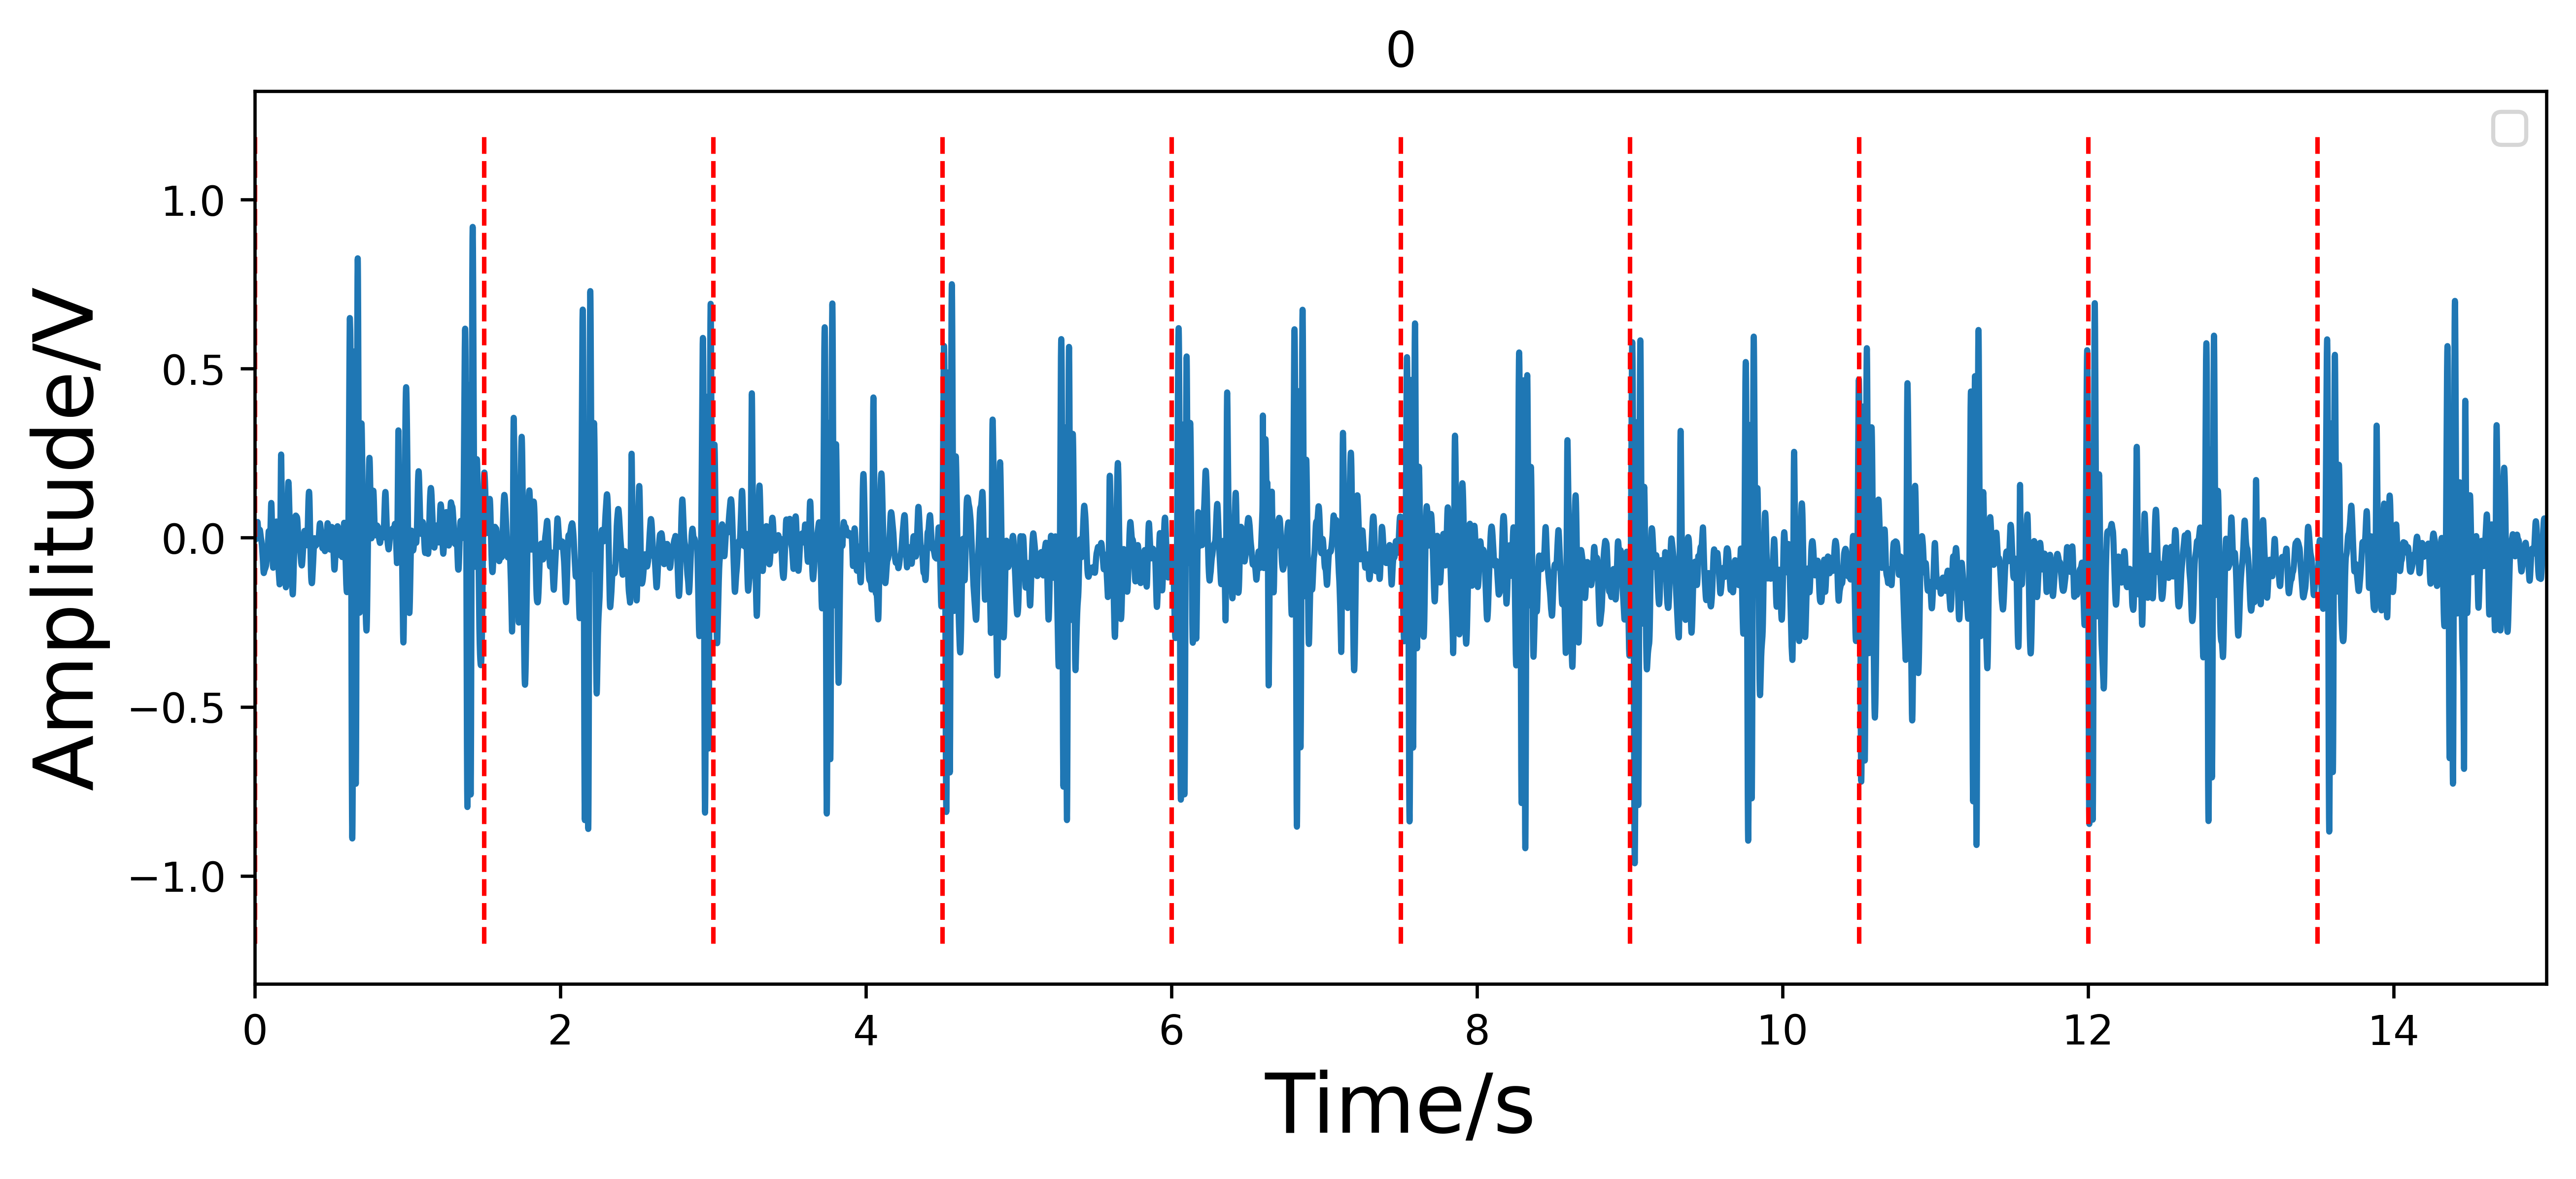
\includegraphics[width=1\linewidth]{figs/disscussion/1.5s.png}
        \caption{Cut with a length of 1.5s}
        \label{FIG:length.a}
    \end{subfigure}\vfill
    % 插入第二张子图
    \begin{subfigure}{.85\linewidth}
        \centering
        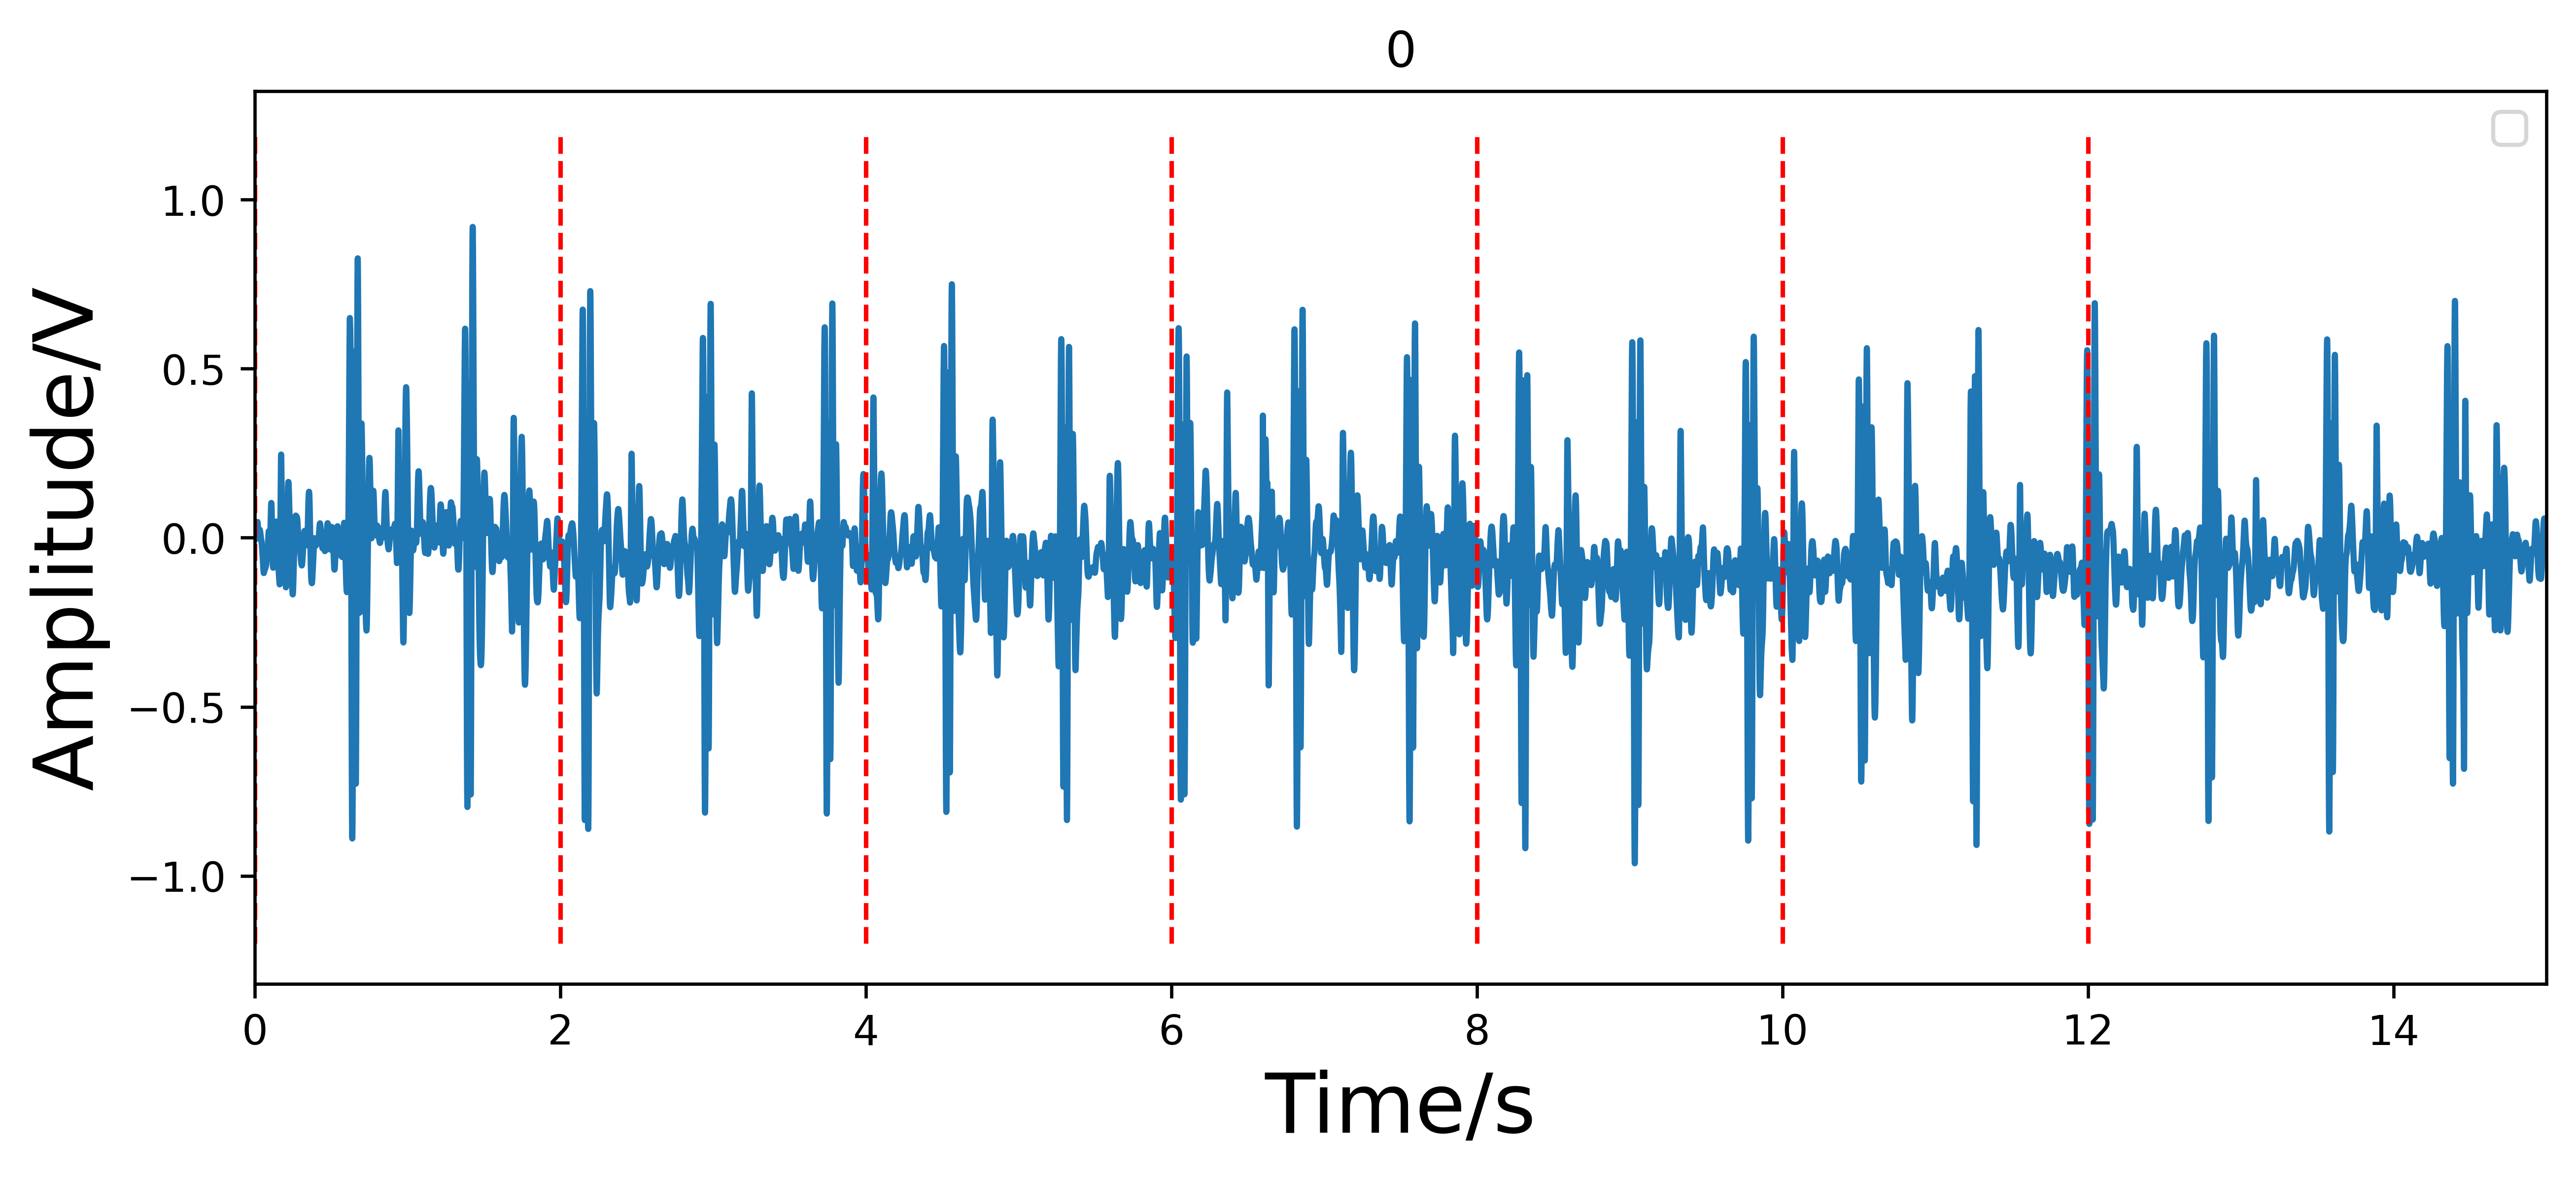
\includegraphics[width=1\linewidth]{figs/disscussion/2s.png}
        \caption{Cut with a length of 2s}
        \label{FIG:length.b}
    \end{subfigure}\vfill
    \begin{subfigure}{.85\linewidth}
        \centering
        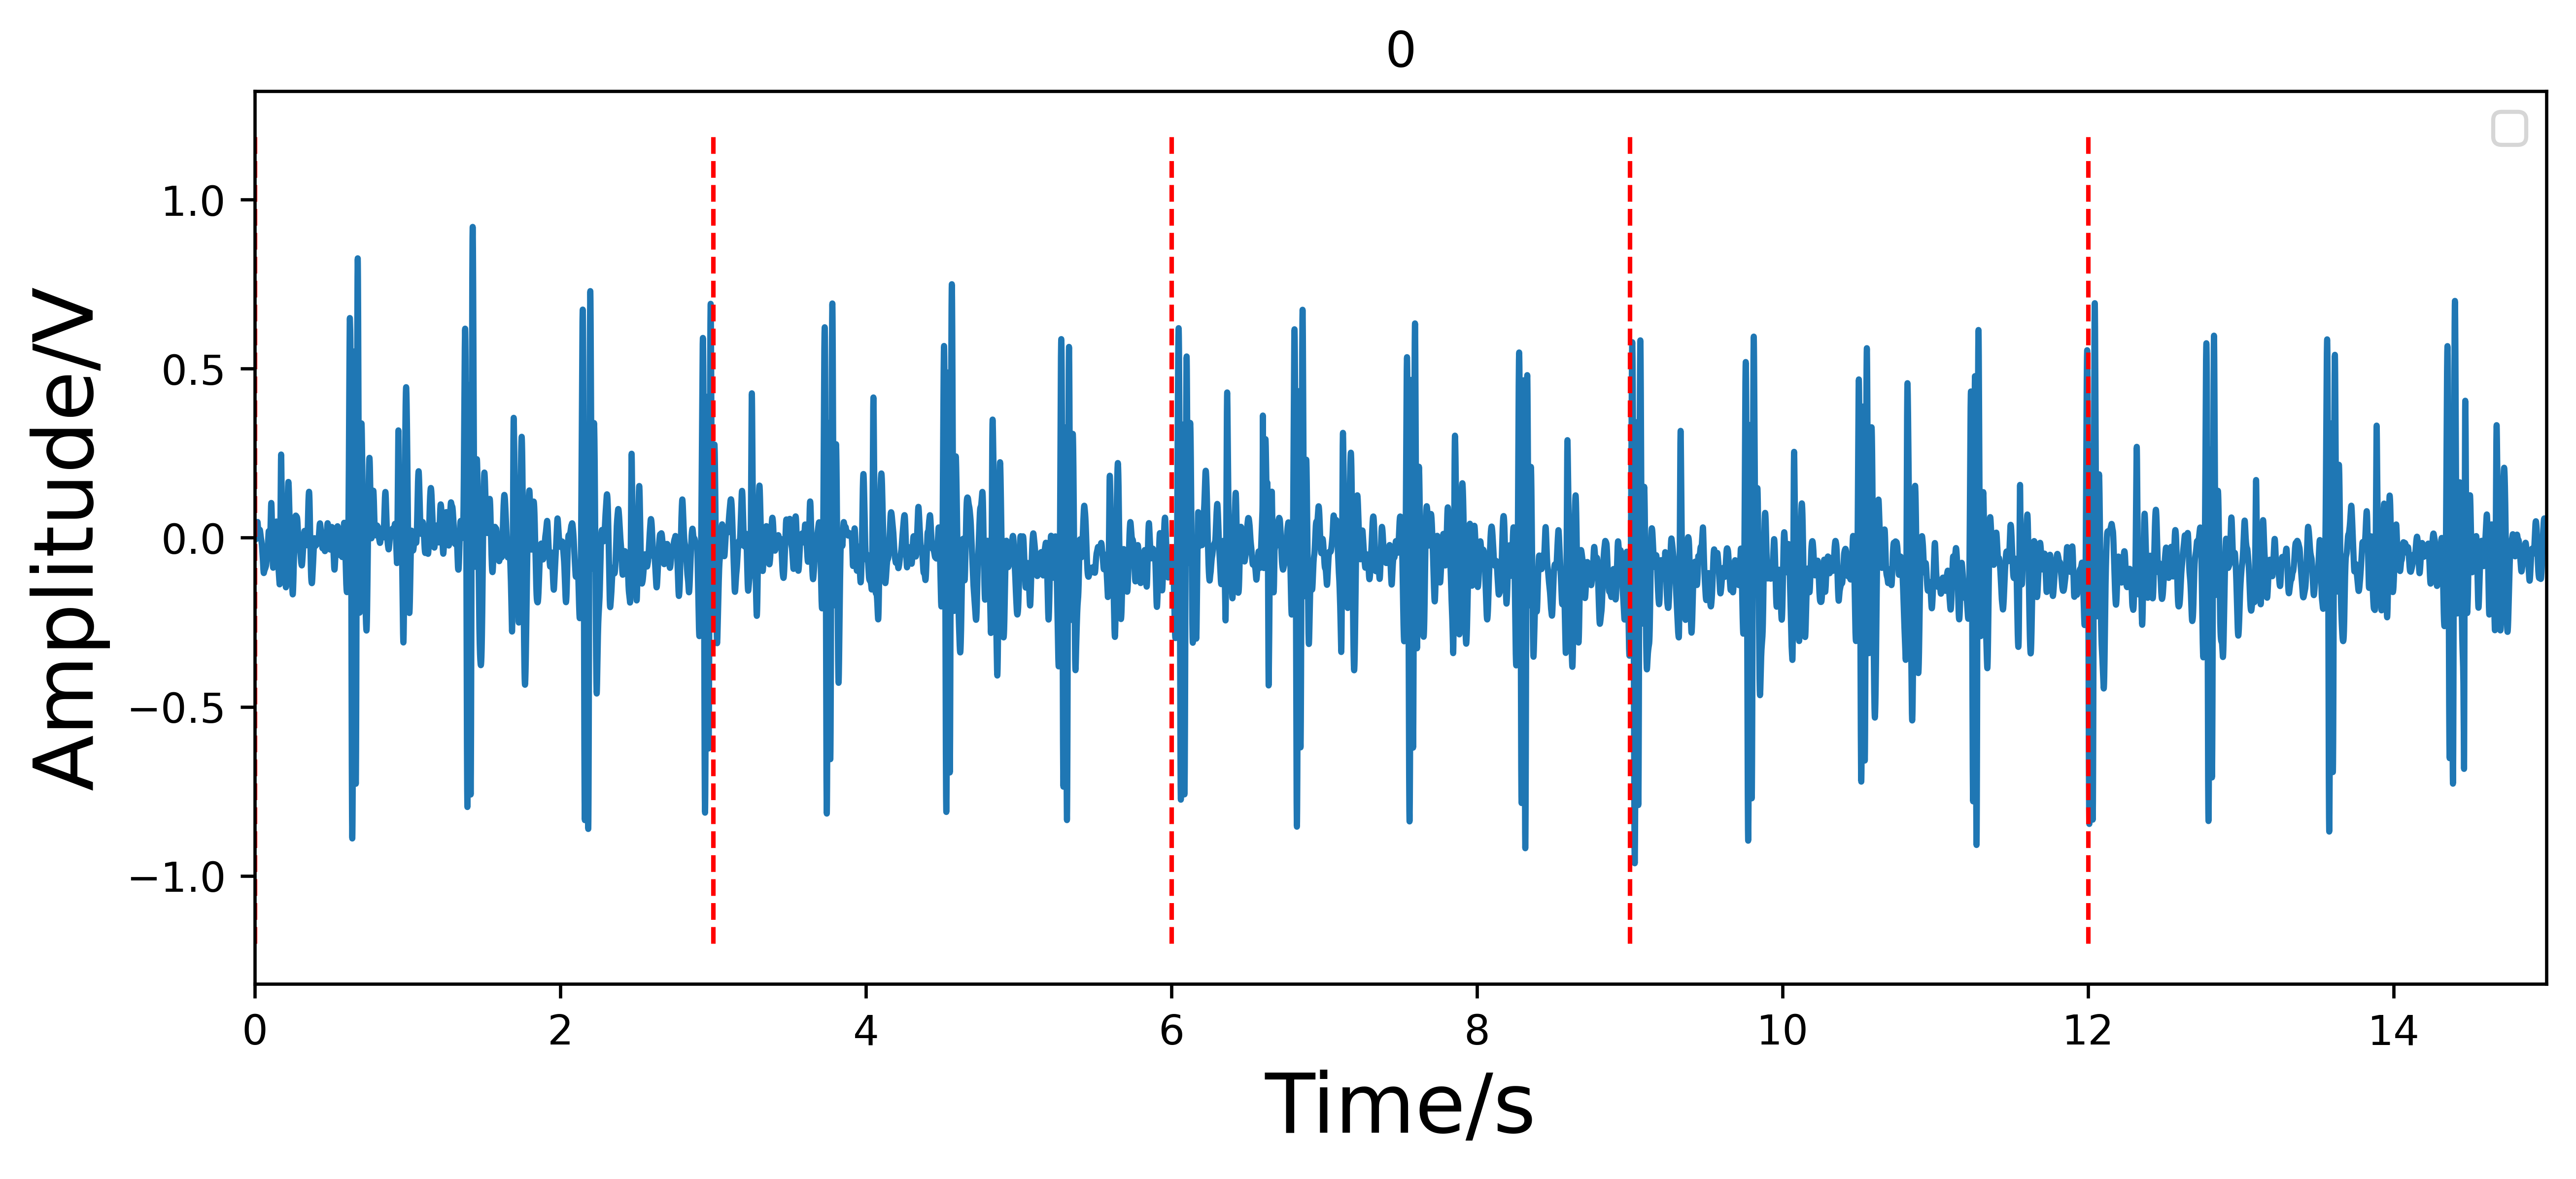
\includegraphics[width=1\linewidth]{figs/disscussion/3s.png}
        \caption{Cut with a length of 3s}
        \label{FIG:length.c}
    \end{subfigure}
\caption{\textbf{Effect of different cutting lengths.} (\textbf{a}) A heart sound is cut with lengths of 1.5s. (\textbf{b}) The same heart sound is cut with lengths of 2s. (\textbf{c}) The same heart sound is cut with lengths of 3s.}
\label{FIG:length}
\end{figure}
\subsection{Results discussion}
\subsubsection{Preprocessing and feature extraction}
This paper conducts an in-depth investigation into the optimal decomposition layers, wavelet bases, and threshold shrinkage functions for the denoising of short heart sounds. Fig.\ref{FIG:wavelet} presents our findings, indicating that a 7-layer decomposition using the $f_{self}$ threshold based on the sym8 wavelet yields the most effective denoising results. It's worth noting that Db6 and sym8 wavelets exhibit similar properties, but sym8, due to its shorter support length and superior energy concentration, is more morphologically aligned with heart sounds.

In contrast to previous studies by Chen \cite{2006Research} and Zhao \cite{2010Research}, this paper employs Signal-to-Noise Ratio (SNR) as the primary metric for evaluating noise reduction, avoiding the limitations of waveform comparison. Additionally, our denoising experiments encompass 26 pathological heart sounds, enhancing the clinical relevance of our findings. Furthermore, in comparison to Cheng \cite{cheng2014denoising}, we propose a new $f_{self}$ construction method that significantly improves SNR (7.8 dB).

As depicted in Fig.\ref{FIG:mfcc}, this study delves into the intricacies of feature extraction, particularly focusing on Mel-spectrum and MFCC. The MFCC feature extraction method for heart sounds possesses the advantage of preserving not only temporal waveform features but also capturing frequency energy distribution. This approach retains valuable information aligned with the Mel scale, which corresponds to human auditory perception.

Fig.\ref{FIG:mfcc.a} illustrates a representation of normal heart sounds, while Fig.\ref{FIG:mfcc.b} showcases an instance of heart sounds from a patient with Mitral Valve Prolapse. Both Mel spectrum and MFCC representations encompass a comprehensive range of waveform characteristics, effectively capturing the intricacies of high-frequency signal features in the form of heat maps.
\begin{figure}[!h]
\centering
    % 插入第一张子图
    \begin{subfigure}{.48\linewidth}
        \centering
        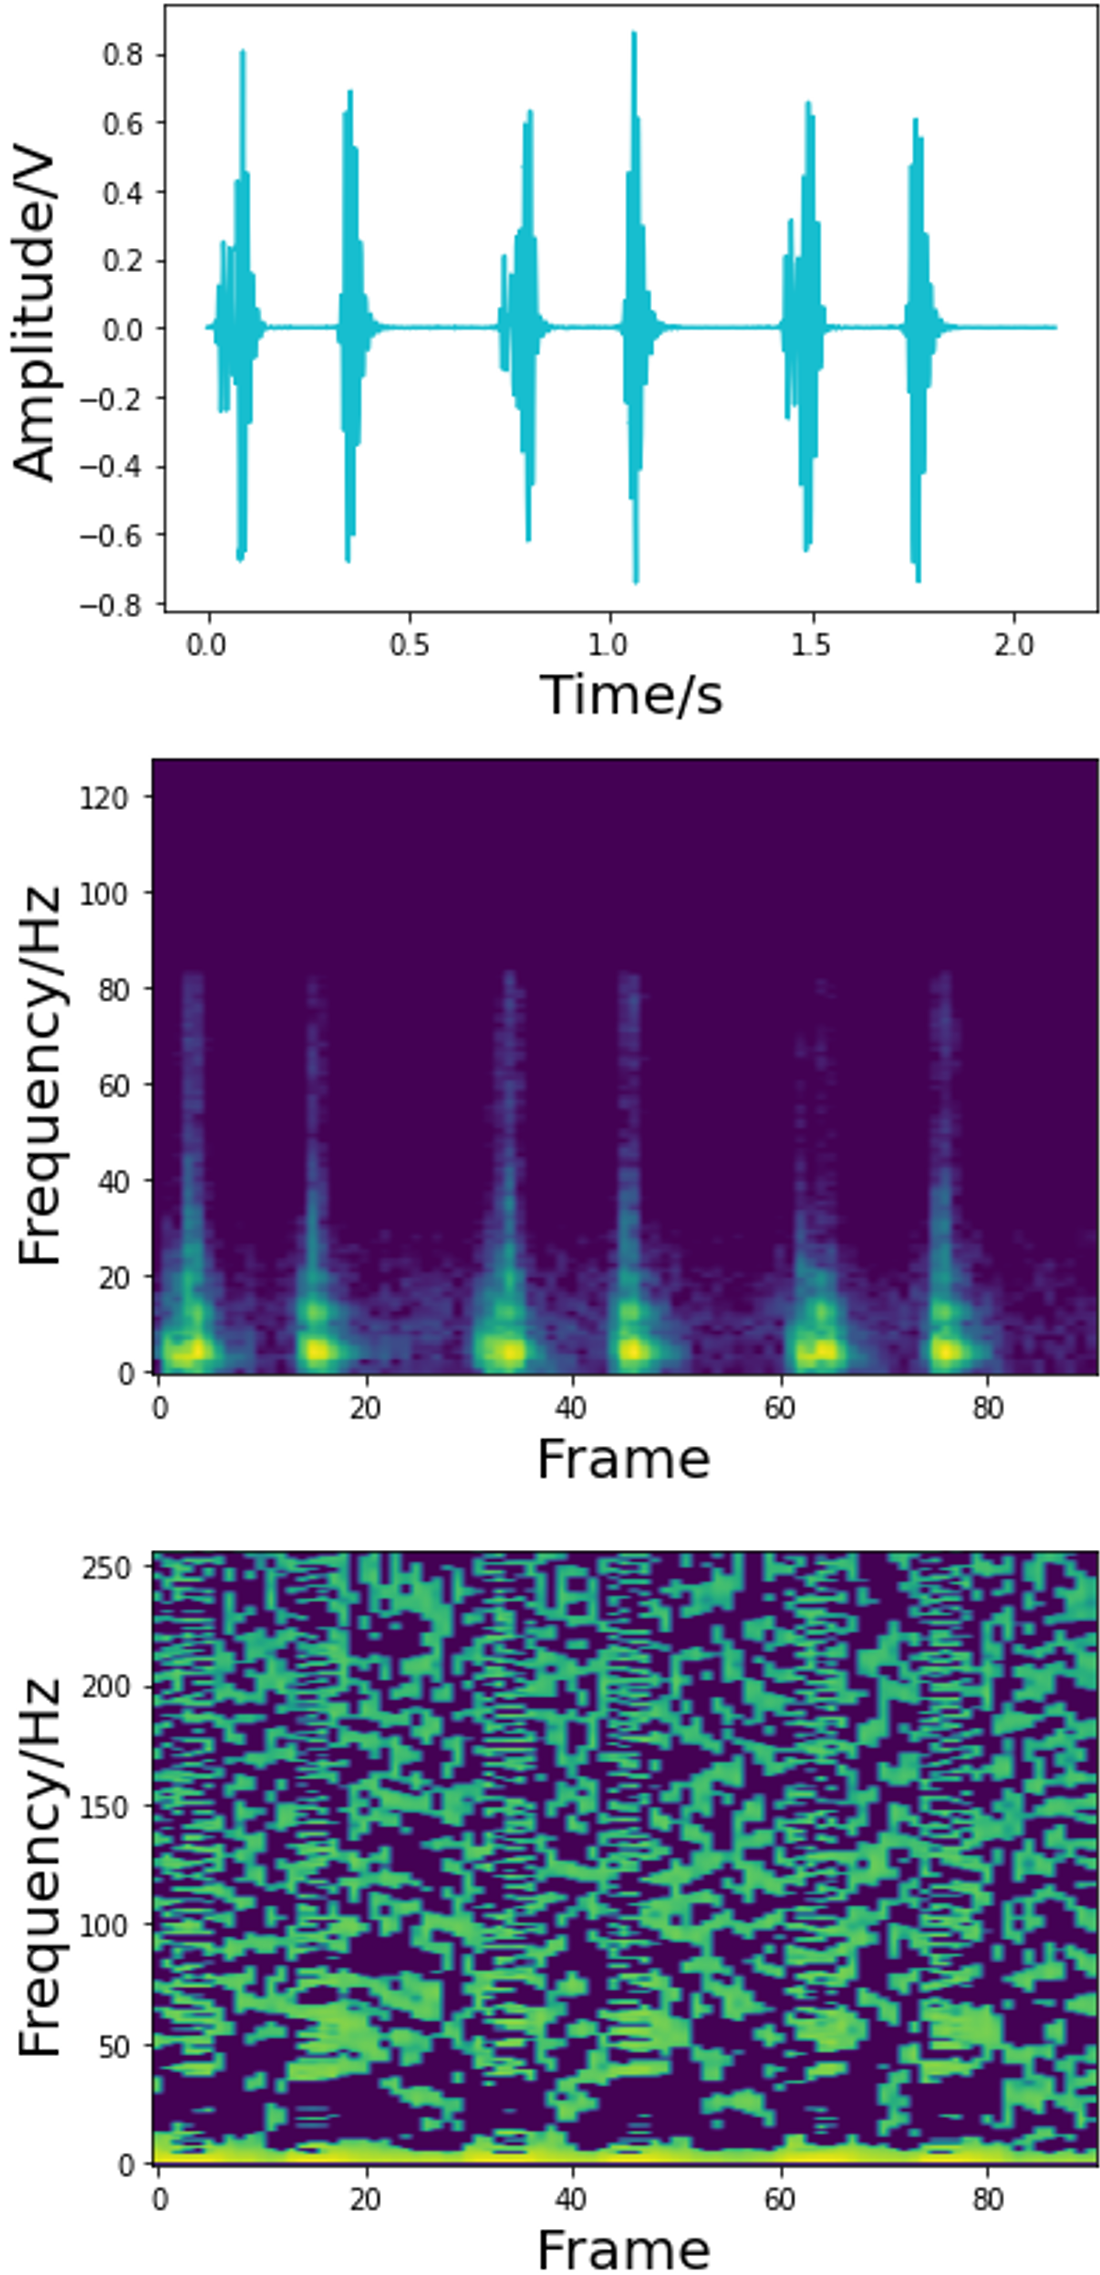
\includegraphics[width=0.99\linewidth]{figs/results/n_mfcc.png}
        \caption{Normal heart sound}
        \label{FIG:mfcc.a}
    \end{subfigure}\hfill
    % 插入第二张子图
    \begin{subfigure}{.48\linewidth}
        \centering
        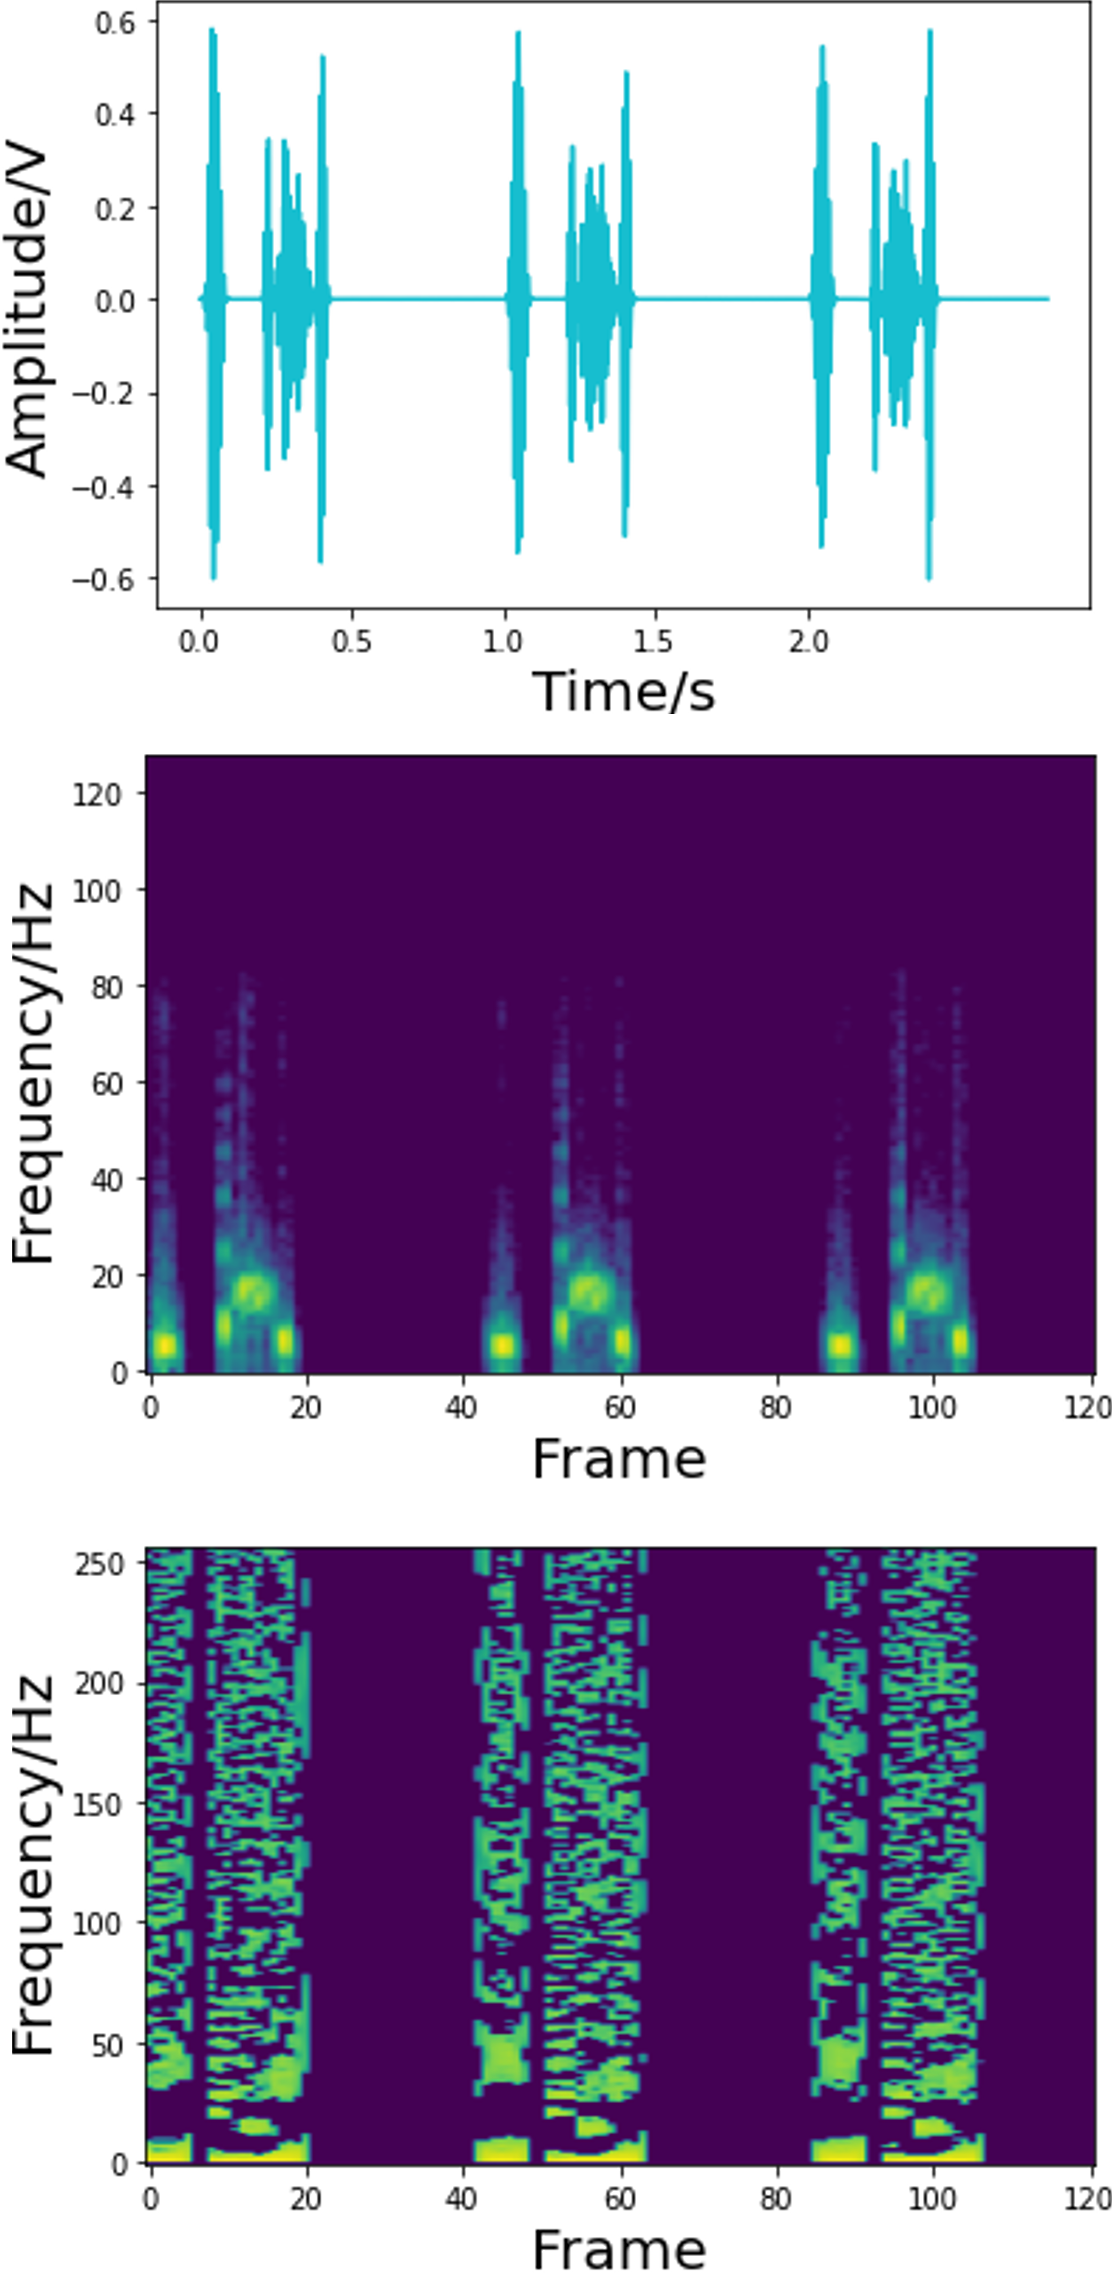
\includegraphics[width=1\linewidth]{figs/results/mvp_mfcc.png}
        \caption{Unhealthy heart sound}
        \label{FIG:mfcc.b}
    \end{subfigure}
\caption{\textbf{Feature extraction result}. (\textbf{a}) Waveform, Mel-spectrum, MFCC of normal heart sound. (\textbf{b}) Waveform, Mel-spectrum, MFCC of unhealthy MVP heart sound.}
\label{FIG:mfcc}
\end{figure}
\subsubsection{Diagnostic performance}
Tab. \ref{tab:HF Diagnosis 10-fold Results} presents the diagnostic outcomes for two heart failure diagnostic datasets and the publicly available Yaseen dataset.

For multi-region fusion auscultation, DenseHF-Net, ResNet-18, and MobileNetV1-28 undergo 10-fold cross-training to calculate average accuracy, sensitivity, specificity, and F1-Score. Among these three models, DenseHF-Net achieves the highest performance, followed by MobileNetV1-28 and ResNet-18. DenseHF-Net attains an accuracy of 99.35\%, 0.64\% higher than ResNet-18 and 0.21\% higher than MobileNetV1-28. In terms of sensitivity, DenseHF-Net records 99.08\%, which is 0.01\% lower than ResNet-18 and 0.92\% lower than MobileNetV1-28. Regarding specificity, DenseHF-Net demonstrates 99.75\%, 1.65\% lower than ResNet-18 and 1.80\% lower than MobileNetV1-28. The F1-Score for DenseHF-Net stands at 99.42\%, 0.83\% higher than ResNet-18 and 0.45\% higher than MobileNetV1-28.

For mitral valve auscultation, DenseHF-Net exhibits an accuracy of 94.41\%, which is 3.08\% higher than ResNet-18 and 3.68\% higher than MobileNetV1-28. The sensitivity of DenseHF-Net is 96.11\%, 3.79\% higher than ResNet-18, and 5.43\% higher than MobileNetV1-28. The specificity for DenseHF-Net reaches 92.00\%, 1.80\% higher than ResNet-18, and 1.20\% higher than MobileNetV1-28. The F1-Score for DenseHF-Net stands at 93.95\%, 2.78\% higher than ResNet-18 and 3.26\% higher than MobileNetV1-28.

Regarding the public Yaseen dataset \cite{son2018classification}, the models exhibit robust generalization abilities for short heart sounds. For the diagnosis of aortic stenosis, mitral regurgitation, mitral stenosis, and mitral valve prolapse, both ResNet-18 and MobileNetV1-28 perform well, achieving accuracies exceeding 82.50\%. However, DenseHF-Net does not perform as well in the diagnosis of mitral regurgitation, mitral stenosis, and mitral valve prolapse, with an accuracy of 63.75\% and an F1-Score of 45.88\%.

Previous researchers have also explored various intelligent algorithms for heart failure diagnosis or prediction, as shown in Tab. \ref{tab:Comparison}. Khade \cite{khade2019system} and Rao \cite{rao2022explainable} predicted heart failure incidence rates based on physiological parameters or medication records. Acharya \cite{acharya2019deep} and Matsumoto \cite{matsumoto2020diagnosing} examined the potential of diagnosing heart failure using ECG or X-ray images. In comparison to Khade \cite{khade2019system} and Rao \cite{rao2022explainable}, this paper offers enhanced medical diagnostic value and interpretability, along with Acharya \cite{acharya2019deep} and Matsumoto \cite{matsumoto2020diagnosing}. When compared to Acharya \cite{acharya2019deep} and Matsumoto \cite{matsumoto2020diagnosing}, this study theoretically boasts superior diagnostic speed, reduced device size, and more suitable application in ambulance settings.

Compared with previous classification research efforts \cite{vepa2009classification, wu2010hidden, rubin2016classifying, arora2021transfer, li2021lightweight, shuvo2021cardioxnet}, this study incorporates several well-established and successful methods, including wavelet denoising, MFCC feature extraction, and the use of CNNs. We address the issue of signal processing and diagnosis in rapid short-duration auscultation. However, it lacks strong generalization capabilities in diagnosing mitral regurgitation, indicating that the model still suffers from overfitting problems. 
Another limitation is the insufficient discussion of subtypes of AHF.

\begin{table*}[!h]
 \caption{Comparison with other researches}
  \label{tab:Comparison}
    \centering
    \begin{tabular}{lcccc}
        \toprule
		 \multicolumn{5}{c}{Comparison with other heart failure researches}\\
        \multicolumn{2}{l}{Authors} & \multicolumn{1}{c}{Database} & \multicolumn{2}{c}{Aim}\\
        \midrule
        \multicolumn{2}{l}{\textbf{Ours}} & \multicolumn{1}{c}{HF-Diagnosis dataset} & \multicolumn{2}{c}{HF diagnosis}\\
        \multicolumn{2}{l}{Khade \cite{khade2019system}} & \multicolumn{1}{c}{Physiological parameters}& \multicolumn{2}{c}{CHF prediction}\\
        \multicolumn{2}{l}{Rao \cite{rao2022explainable}} & \multicolumn{1}{c}{Medication records} & \multicolumn{2}{c}{CHF prediction}\\
        \multicolumn{2}{l}{Acharya \cite{acharya2019deep}} & \multicolumn{1}{c}{ECG} & \multicolumn{2}{c}{HF diagnosis}\\
        \multicolumn{2}{l}{Matsumoto \cite{matsumoto2020diagnosing}} & \multicolumn{1}{c}{X-Ray Images} & \multicolumn{2}{c}{HF diagnosis} \\
        \toprule
		 \multicolumn{5}{c}{Comparison with other heart sound researches}\\
        Authors & Feature extraction & Classification method & Databases & Acc$(\%)$ \\
                \midrule
        \textbf{Ours} & MFCC & DenseHF-Net & Mitral valve auscultation dataset & 94.41 \\
        Vepa \cite{vepa2009classification} & STFT, DWT & kNN, MLP, SVM & Normal, systolic, diastolic records& 95.2\\
        Wu \cite{wu2010hidden} & MFCC & HMM & 325 cycles of 10-type& 95.08 \\
        Rubin \cite{rubin2016classifying} & MFCC & CNN & PhysioNet 2016& 95.2\\
        Arora \cite{arora2021transfer} & STFT & CNN & PhysioNet 2016& 89.04\\
        Li \cite{li2021lightweight} & STFT & CNN & PhysioNet 2016 & 85\\
        Shuvo \cite{shuvo2021cardioxnet} & Time-invariant features &CNN & Yaseen database& 99.6\\
        \bottomrule
    \end{tabular}
\end{table*}
